\date{03.10.2024}

Exemplo: Localize no $\mathbb{R}^2$ os pontos que satisfazem:
\begin{itemize}
    \item[a. ] $(x-1)^2 + (y-2)^2 = 1 $ e $z = 3$
    \item[b. ] $(x-4)(z-2) = 0$ 
        R: Note que $(x-4)(z-2) = 0$ ocorre $\leftrightarrow x -4 = 0$ ou $z-2=0 \leftrightarrow x = 4$ ou $z=2$             
\end{itemize}

Exemplo: Srjam P=(-5,2,3) e Q=(3,4,-1). Determine a esuqeção da esfera que tem $\overline{PQ}$ \\
Pmédio = $\left(\frac{x_1+x_2}{2}, \frac{y_1+y_2}{2}, \frac{z_1+z_2}{2} \right) $
%grafico 2d% \\
$P_u = u + \frac{1}{2}v = (x_1,y_1)+ \frac{1}{2}(x_2-x_1)(y_2 - y_1) = \left(\frac{x_2+x}{2} , \frac{y_2+y_1}{2} \right)$

\subsection{Vetores}
\textbf{Definição:}
Dados 2 pontos A ou B em $\mathbb{R}^3$ ou $\mathbb{R}^2$, o segmento orientado a $\overrightarrow{AB}$ é o segmento com ponto incicial A, ponto final V e orientado de $A \rightarrow B$.
%grafico 3%
\textbf{Definição:}
Um segmento não nulo de $\overrightarrow{AB}$ é equivalente a $\overrightarrow{CD}$ ou $\overrightarrow{AB}$ e $\overrightarrow{CD}$ tem o mesmo comprimento e direção e sentido %grafico acima%.
Dados dois segmentos orientados $\overrightarrow{AB}$ e $\overrightarrow{BC}$, definimos: a soma de $\overrightarrow{AB} + \overrightarrow{BC} = \overrightarrow{AC}$
Em geral, sejam u e v dois segmentos orientados. Para determina u+v, podemos seguir uma das duas abordagens:
\begin{figure}[!h]
    \centering
    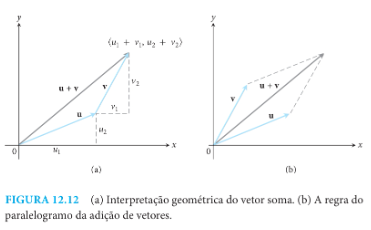
\includegraphics{graficosoma.png}
    \caption{Descrição da imagem}
    \label{fig:exemplo}
\end{figure}

Dado um segmento u de reta orientado $\overrightarrow{AB}$, existe um segmento de reta orientado $\overrightarrow{v}$, equiavalente a $\overrightarrow{AB}$ e com ponto inicial em (0,0,0). Para especificiar $\overrightarrow{v}$ precisamos apenas fornecer as coordenadas de um ponto final (a,b,c).
De modo geral, o vetor $\overrightarrow{v} = <x,y,z>$ é definido como o segmento de reta orientada com ponto inicial em (0,0,0) e ponto final $(x,y,z)$.


\textbf{Observação:} Sejam $u=<x,y,z>$ e $v=<x_2,y_2,z_2>$. Então: $u=v \leftrightarrow \{x_1 = x_2 \\ y_1 = y_2 \\ z_1 = z_2 \}$


\textbf{Observação:} Dados $A=(x_1,y_1,z_1)$ e $B=(x_2,y_2,z_2)$, o vetor equivalente a $\overrightarrow{AB}$ (ou vetor com representação $\overrightarrow{AB}$). $v = <x_2-x_1, y_2-y_1, z_2-z_1>$.


Exemplo: Dados $A=(1,4,0)$, $B=(-1,1,-1)$ e $C = (3,5,-10)$, encontre o vetor $\overrightarrow{v}$ equivalente a $\overrightarrow{AB}$ e as coordenadas do ponto D tal que $\overrightarrow{CD} = \overrightarrow{v}$
Solução: Segue se $v = <x_2-x_1, y_2-y_1, z_2-z_1>$ que $v=<-1-(1), 1-(4), -1-(0)> = <-2,-3,-1>$. Queremos encontrar D=(a,b,c) de tal modo que $\overrightarrow{v}$ seja equiavalente a $\overrightarrow{CD}$.
$<-2,-3,-1> = <a-3,b-5,c-(-10)> \leftrightarrow {a-3 = -2 \rightarrow a=1} {b-5 = -3 \rightarrow b=2} {c+10 = -1 \rightarrow c=-11}$ 

\subsubsection{Operação com Vetores}
\paragraph{Soma}: Sejam $\overrightarrow{u} = <x_1,y_1,z_1>$ e $\overrightarrow{v} = <x_2,y_2,z_2>$. Definimos a soma $\overrightarrow{u} + \overrightarrow{v}$ por $\overrightarrow{u} + \overrightarrow{v} = <x_1+x_2, y_1+y_2, z_1+z_2>$.
\paragraph{Produto Escalar}: Seja $k \in \mathbb{R}$ e $\overrightarrow{u} = <x_1,y_1,z_1>$. Definimos o produto $k*\overrightarrow{u} = <kx_1, ky_1, kz_1>$.
\paragraph{Comprimento}: O comprimento de $\overrightarrow{u} = <x_1, y_1, z_1>$ é $|| \overrightarrow{u} || = \sqrt{x_1^2, y_1^2, z_1^2}